% Book 4, Year 2, chapter 5 -- The standard library: containers, iterators and algorithms.
% Provenance (never printed): sources/book4/BRIEFS.md, chapter 5.
\chapter{The Standard Library: Containers, Iterators and Algorithms}\label{ch:b2:cpp-standard-library}

The town library wants to know which words come back most often in the titles of its 80 books. Last year that
meant a hash table written by hand. The C++ standard library has one, and a balanced search tree, and a sort; the
whole count is the loop below, and its heart is the line \code{count[word]++}.

\omcode{code/bachelor-2/05-cpp-standard-library/listings/words.hpp}{18}{32}{Counting words with a
\code{std::map}}\label{lst:b2:cpp-standard-library:words}

\omoutput{code/bachelor-2/05-cpp-standard-library/outputs/run_word_count.txt}{The 262 words of the titles, and the
most frequent.}\label{out:b2:cpp-standard-library:word-count}

\code{count[word]} finds the word in a search tree and, if it is missing, inserts it with the value 0;
\code{by_frequency} copies the pairs into a vector and sorts it by count. No allocation, no rebalancing, no hashing
was written. This chapter is about knowing what the library did for us, and what it costs.

\begin{recall}
Book 3 built the structures this library packages: the dynamic array with its amortised constant append, the
linked list, the hash table with its load factor, the balanced search trees, among them the red-black tree, and the
binary heap; it also used an \emph{iterator}, an object that designates a position in a collection and moves to
the next one. \cref{ch:b2:cpp-templates}: every \omterm{def:b2:cpp-standard-library:container}{container} and algorithm below is a \omterm{def:b2:cpp-templates:template}{template}.
\end{recall}

\section{Sequence containers}\label{sec:b2:cpp-standard-library:sequence}

\begin{definition}[Container]\label{def:b2:cpp-standard-library:container}
A \emph{container}\index{container (C++)} is a \omterm{def:b2:cpp-templates:template}{class template} of the standard library that owns a collection of
elements of one type, and manages their memory. A \emph{sequence container}\index{sequence container} keeps the
elements in the order the program puts them: \code{std::array}, \code{std::vector}, \code{std::deque},
\code{std::list}. An \emph{associative container}\index{associative container} keeps them sorted by a key, in a
balanced search tree: \code{std::set}, \code{std::map}. An \emph{unordered container}\index{unordered container}
places them by the hash of their key, in a hash table: \code{std::unordered_set}, \code{std::unordered_map}.
\end{definition}

The four sequence \omterm{def:b2:cpp-standard-library:container}{containers} are four structures of Book 3. \code{std::array<T, N>} is a C array of fixed size
wrapped in a class; \code{std::vector<T>} the dynamic array; \code{std::list<T>} the doubly linked list;
\code{std::deque<T>} (double-ended queue) a table of pointers to fixed-size blocks, which grows at both ends without
moving its elements. The program below gives each of them the same four integers and measures two things: the size
of the object itself, and the distance between the first two elements in memory.

\omcode{code/bachelor-2/05-cpp-standard-library/listings/containers.cpp}{8}{32}{Four sequence \omterm{def:b2:cpp-standard-library:container}{containers} side by
side}\label{lst:b2:cpp-standard-library:containers}

\omoutput{code/bachelor-2/05-cpp-standard-library/outputs/containers.txt}{The array holds its elements inside the
object; the others hold pointers.}\label{out:b2:cpp-standard-library:containers}

The \code{array} object is its 16 bytes of elements. A \code{vector} is three pointers, 24 bytes, whatever its size,
and its elements are side by side on the heap, 4 bytes apart. A \code{list} is two pointers and a count, and each
element lives in a node of its own, with a pointer to the next node and one to the previous: 4 bytes of data in
a 32-byte block of the allocator, the nodes here allocated one after the other. The \code{deque}'s 80 bytes hold
the table and the positions of both ends; its elements are contiguous inside each block.

\section{Associative and unordered containers}\label{sec:b2:cpp-standard-library:associative}

A \code{std::map<K, V>} stores pairs of a key and a value, sorted by key; it is the dictionary of Book 3 built on
a balanced search tree. A \code{std::unordered_map<K, V>} offers the same operations on a hash table. Below, both
receive eight street names of the town, in the same order.

\omcode{code/bachelor-2/05-cpp-standard-library/listings/buckets.cpp}{9}{32}{The same eight keys in a tree and in a
hash table}\label{lst:b2:cpp-standard-library:buckets}

\omoutput{code/bachelor-2/05-cpp-standard-library/outputs/buckets.txt}{The map visits the keys in alphabetical order,
the hash table in its own.}\label{out:b2:cpp-standard-library:buckets}

% ledger: b2:map-complexity
The standard does not name the tree behind \code{std::map}: it requires searches, insertions and removals in
logarithmic time, and in practice the libraries use a red-black tree. The figure shows the one the eight insertions
built, as the library of the compiler used here really stores it.

\begin{omfigure}
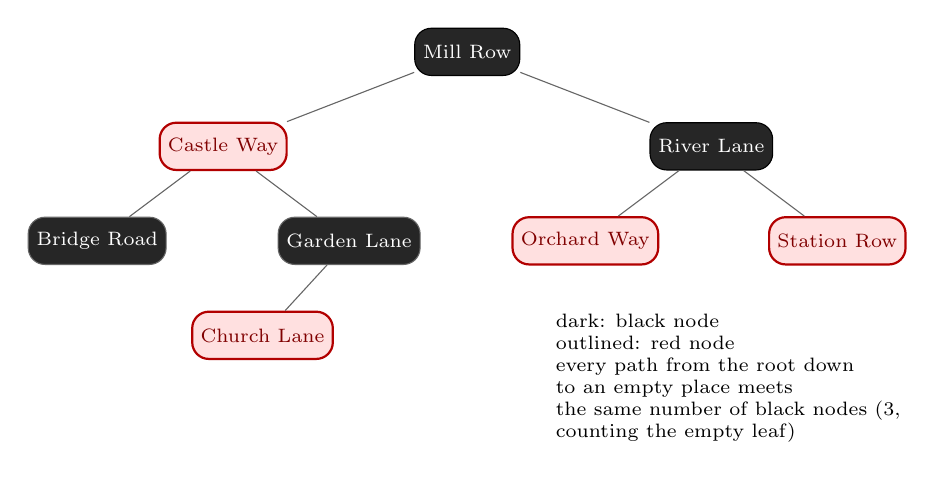
\begin{tikzpicture}[font=\scriptsize,
    bk/.style={draw, rounded corners=6pt, fill=black!85, text=white, minimum height=6mm, inner sep=3pt},
    rd/.style={draw=red!70!black, thick, rounded corners=6pt, fill=red!12, text=red!50!black, minimum height=6mm, inner sep=3pt},
    level distance=12mm, level 1/.style={sibling distance=62mm}, level 2/.style={sibling distance=32mm},
    level 3/.style={sibling distance=22mm}, edge from parent/.style={draw, black!60}]
\node[bk] {Mill Row}
  child {node[rd] {Castle Way}
    child {node[bk] {Bridge Road}}
    child {node[bk] {Garden Lane}
      child {node[rd] {Church Lane}}
      child[missing] {}}}
  child {node[bk] {River Lane}
    child {node[rd] {Orchard Way}}
    child {node[rd] {Station Row}}};
\node[anchor=north west, align=left, font=\scriptsize] at (1.0,-3.2) {dark: black node\\ outlined: red node\\
  every path from the root down\\ to an empty place meets\\ the same number of black nodes (3,\\
  counting the empty leaf)};
\end{tikzpicture}
\par\smallskip{\small The red-black tree of \cref{lst:b2:cpp-standard-library:buckets}'s \code{std::map}, inserted
in the order Mill Row, Bridge Road, Station Row, Castle Way, River Lane, Garden Lane, Orchard Way, Church Lane. No
red node has a red child, and the in-order walk, left subtree, node, right subtree, gives the alphabetical order of
the output. The shape was read from the library's own nodes and recomputed by the insertion algorithm of Book 3.}
\end{omfigure}

% ledger: b2:unordered-complexity
% ledger: b2:unordered-max-load
The hash table has 13 buckets for 8 elements, a load factor of $8/13 \approx 0.62$. Its maximum is 1.0: one more
element than buckets, and the table allocates more buckets and moves every element to its new bucket, which is a
\emph{rehash}. Bucket 11 holds three names and bucket 12 two, while eight buckets are empty: with a good hash
function, collisions are the normal case, not an accident. Search, insertion and removal take constant time on
average, and linear time in the worst case, when the keys share one bucket.

\begin{omfigure}
\begin{tikzpicture}[font=\scriptsize, k/.style={draw, rounded corners=2pt, fill=omDef!10, inner sep=2.5pt, minimum height=4.6mm, minimum width=19mm}]
\foreach \b in {0,...,12} {
  \node[cell, minimum width=8mm, minimum height=4.6mm] (b\b) at (0,-0.52*\b) {\b};
}
\node[font=\scriptsize\bfseries] at (0,0.55) {bucket};
\foreach \b/\names in {2/{River Lane}, 8/{Mill Row}, 10/{Church Lane}, 11/{Orchard Way,Garden Lane,Bridge Road},
                      12/{Castle Way,Station Row}} {
  \coordinate (prev) at (b\b.east);
  \foreach \n [count=\i] in \names {
    \node[k, anchor=west] (n\b-\i) at ($(b\b.east) + (0.6 + 2.5*\i - 2.5, 0)$) {\n};
    \draw[ptr] (prev) -- (n\b-\i.west);
    \coordinate (prev) at (n\b-\i.east);
  }
}
\node[anchor=west, align=left, font=\scriptsize] at (8.4,-1.6) {8 elements, 13 buckets\\ load factor 0.62\\[2pt]
  a lookup hashes the key, picks\\ its bucket, and compares the key\\ with that bucket's elements only};
\end{tikzpicture}
\par\smallskip{\small The 13 buckets of the \code{unordered_map}, from the output of
\cref{lst:b2:cpp-standard-library:buckets}, drawn as one chain per bucket. The library actually threads every
element on a single list and keeps, for each bucket, where its stretch of that list begins, which is why the
iteration order of the output visits the buckets in no visible order.}
\end{omfigure}

\section{Iterators}\label{sec:b2:cpp-standard-library:iterators}

Every \omterm{def:b2:cpp-standard-library:container}{container} gives access to its elements by iterators, which the algorithms of the next section take as
arguments: an algorithm written for iterators works on every \omterm{def:b2:cpp-standard-library:container}{container}.

\begin{definition}[Iterator range]\label{def:b2:cpp-standard-library:iterator}
An \emph{iterator range}\index{iterator range} is a pair of iterators \code{first} and \code{last} of one
collection, designating the elements from \code{first} up to, but not including, \code{last}: the half-open range
$[\code{first}, \code{last})$. It is empty when \code{first == last}. \code{c.begin()} designates the first element
of a \omterm{def:b2:cpp-standard-library:container}{container} \code{c} and \code{c.end()} the position just after the last one, which may be compared with but not
read.
\end{definition}

Half-open ranges make empty ranges natural and lengths a subtraction, $\code{last} - \code{first}$, and split well:
$[a, m)$ and $[m, b)$ cover $[a, b)$ with no overlap. Not every iterator can do everything a pointer can. A list
iterator moves one node at a time and cannot jump by 1000; a map iterator walks the tree in order.

\begin{definition}[Iterator category]\label{def:b2:cpp-standard-library:category}
The \emph{iterator categories}\index{iterator category} are nested sets of operations. An \emph{input} iterator
can be read and advanced once, in one pass. A \emph{forward} iterator can be copied and its range traversed several
times. A \emph{bidirectional} iterator can also move back (\code{--it}). A \emph{random-access} iterator can also
jump (\code{it + k}), subtract and compare in constant time. A \emph{contiguous} iterator designates elements
adjacent in memory. Each category has a C++20 concept, such as \code{std::random_access_iterator}.
\end{definition}

\begin{omfigure}
\begin{tikzpicture}[font=\scriptsize, cat/.style={draw=omDef!60!black, rounded corners=3pt, fill=omDef!12,
    minimum width=26mm, minimum height=7mm, font=\scriptsize\bfseries}]
\foreach \i/\name/\ops/\ex in {
  0/input/{read \texttt{*it}, advance \texttt{++it}, one pass}/{\texttt{std::istream\_iterator}},
  1/forward/{copy it, traverse the range again}/{\texttt{std::forward\_list}, \texttt{std::unordered\_map}},
  2/bidirectional/{move back, \texttt{-{}-it}}/{\texttt{std::list}, \texttt{std::map}, \texttt{std::set}},
  3/random access/{\texttt{it + k}, \texttt{it2 - it}, \texttt{it < it2}, in constant time}/{\texttt{std::deque}},
  4/contiguous/{the elements are adjacent in memory}/{\texttt{std::vector}, \texttt{std::array}, pointers}} {
  \node[cat] (c\i) at (0,-1.05*\i) {\name};
  \node[anchor=west, align=left] at (1.6,-1.05*\i) {adds: \ops\\ \textcolor{black!60}{e.g.\ \ex}};
}
\foreach \i [evaluate=\i as \j using int(\i-1)] in {1,...,4}
  \draw[ptr] (c\i.north) -- node[left, font=\tiny, text=black!60] {is also} (c\j.south);
\end{tikzpicture}
\par\smallskip{\small The \omterm{def:b2:cpp-standard-library:category}{iterator categories}, each below the one it refines: a random-access iterator is also a
bidirectional one, and so on. An algorithm states the weakest category it needs; \code{std::sort} needs random
access, so a \code{std::list} cannot be given to it and has a \code{sort} member of its own.}
\end{omfigure}

An iterator holds a pointer into the \omterm{def:b2:cpp-standard-library:container}{container}'s memory, and some operations move that memory.

\begin{definition}[Iterator invalidation]\label{def:b2:cpp-standard-library:invalidation}
An operation on a \omterm{def:b2:cpp-standard-library:container}{container} \emph{invalidates}\index{iterator invalidation} an iterator, a pointer or a reference
to its elements when, after the operation, using it is undefined behaviour. The standard states, for each operation
of each \omterm{def:b2:cpp-standard-library:container}{container}, which ones it invalidates.
\end{definition}

% ledger: b2:vector-insert
For a \code{vector}, an insertion that exceeds the capacity reallocates and \omterm{def:b2:cpp-standard-library:invalidation}{invalidates} everything; one that does
not \omterm{def:b2:cpp-standard-library:invalidation}{invalidates} the positions from the insertion point on. For a \code{list} or a \code{map}, an insertion
\omterm{def:b2:cpp-standard-library:invalidation}{invalidates} nothing and an erasure only the erased element's iterators, since no other node moves. For an
\code{unordered_map}, an insertion that causes a rehash \omterm{def:b2:cpp-standard-library:invalidation}{invalidates} every iterator, but no pointer or reference to
an element, because the nodes do not move: only the bucket table is rebuilt. The program below breaks the
\code{vector} rule.

\omcode{code/bachelor-2/05-cpp-standard-library/listings/invalidation.cpp}{8}{13}{Renewing the loans due in more than
ten days, in the loop that reads them}\label{lst:b2:cpp-standard-library:invalidation}

\omoutput[2-9,14-15,24-24,38-38]{code/bachelor-2/05-cpp-standard-library/outputs/run_invalidation.txt}{A read of
freed memory, staged: the block was freed by the \code{push_back}.}\label{out:b2:cpp-standard-library:invalidation}

The range-\code{for} keeps an iterator \code{it} and the end iterator, both pointing into the vector's first block.
At 12 days, \code{push_back} finds the vector full, allocates a block twice as large, moves the four elements and
frees the old block; the loop then advances \code{it}, still in the old block, and reads freed memory. Without the
sanitizer the program would print garbage or nothing, depending on what reused the block. The fixes: collect the
renewals in a second vector and append them after the loop, or loop on an index, rereading \code{due[i]} each time.

\section{Generic algorithms and lambda expressions}\label{sec:b2:cpp-standard-library:algorithms}

\begin{definition}[Generic algorithm]\label{def:b2:cpp-standard-library:algorithm}
A \emph{generic algorithm}\index{generic algorithm} of the standard library is a \omterm{def:b2:cpp-templates:template}{function template}, declared in
\code{<algorithm>} or \code{<numeric>}, that works on an \omterm{def:b2:cpp-standard-library:iterator}{iterator range} rather than on a \omterm{def:b2:cpp-standard-library:container}{container}, and requires of
its iterators a category: \code{std::find} needs input iterators, \code{std::sort} random-access ones. Algorithms
never add or remove elements of the \omterm{def:b2:cpp-standard-library:container}{container}: they only read, write or reorder through the iterators.
\end{definition}

Most algorithms take an operation as an argument: what \emph{long} means for \code{count_if}, what \emph{before}
means for \code{sort}. The operation is usually written in place.

\begin{definition}[Lambda expression, capture]\label{def:b2:cpp-standard-library:lambda}
A \emph{lambda expression}\index{lambda expression} \code{[captures](parameters) { body }} creates an unnamed
function object, an object of a class generated by the compiler whose \code{operator()} runs the body. Its
\emph{captures}\index{capture (lambda)} list the local variables of the enclosing function the body uses:
\code{[x]} stores a copy of \code{x} in the object, \code{[&x]} a reference to it, \code{[=]} and \code{[&]} capture
every variable the body uses, by copy or by reference.
\end{definition}

\omcode{code/bachelor-2/05-cpp-standard-library/listings/lambdas.cpp}{9}{29}{Counting, finding, summing, sorting and
searching}\label{lst:b2:cpp-standard-library:lambdas}

\omoutput{code/bachelor-2/05-cpp-standard-library/outputs/lambdas.txt}{25 comparisons of the sort counted through a
captured reference.}\label{out:b2:cpp-standard-library:lambdas}

The comparison counter needs a reference capture: a copy would count in the lambda object's own variable, and the
sort copies its comparator, so \code{calls} would stay 0. \code{std::lower_bound} searches a sorted range by
halving it.

% ledger: b2:lower-bound-comparisons
\begin{proposition}[Comparisons of a binary search]\label{prop:b2:cpp-standard-library:lower-bound}
On a sorted range of $n \geq 1$ elements, \code{std::lower_bound} returns the first position whose element is not
less than the key, after at most $\lfloor \log_2 n \rfloor + 1$ comparisons.
\end{proposition}

\begin{proof}
The algorithm keeps a range of length $\ell$, initially $n$, that contains the answer's position or ends just
before it. With $h = \lfloor \ell / 2 \rfloor$, it compares the element at offset $h$ with the key: if it is less,
the answer lies after it and the range becomes the last $\ell - h - 1$ elements; otherwise the answer is at most
this position and the range becomes the first $h$. Both new lengths are at most $\lfloor \ell / 2 \rfloor$. After
$k$ comparisons the length is at most $\lfloor n / 2^k \rfloor$, which is 0 as soon as $2^k > n$, that is for
$k = \lfloor \log_2 n \rfloor + 1$; a range of length 0 needs no comparison and designates the answer.
\end{proof}

C++20 adds \emph{ranges}: the algorithms of \code{std::ranges} accept a whole \omterm{def:b2:cpp-standard-library:container}{container}, and \emph{views} compose
lazy transformations with \code{|}, computed only when the loop asks for the next element.

\omcode{code/bachelor-2/05-cpp-standard-library/listings/ranges.cpp}{9}{20}{Views composed with
\code{|}}\label{lst:b2:cpp-standard-library:ranges}

\omoutput{code/bachelor-2/05-cpp-standard-library/outputs/ranges.txt}{Filtered, transformed, reversed and cut: no
intermediate vector was built.}\label{out:b2:cpp-standard-library:ranges}

\omterm{def:b2:cpp-standard-library:container}{Containers} and algorithms combine: a map from each member to the vector of that member's loans groups the town's
400 loans in one loop, and \code{count_if} with a lambda counts the late ones (returned after the due date, or
still out after it at the end of 2025).

\omcode{code/bachelor-2/05-cpp-standard-library/listings/loans_by_member.cpp}{10}{27}{The loans grouped by
member}\label{lst:b2:cpp-standard-library:loans}

\omoutput{code/bachelor-2/05-cpp-standard-library/outputs/run_loans.txt}{The five busiest
borrowers.}\label{out:b2:cpp-standard-library:loans}

\section{Complexity guarantees and measurement}\label{sec:b2:cpp-standard-library:guarantees}

\begin{definition}[Complexity guarantee]\label{def:b2:cpp-standard-library:guarantee}
A \emph{complexity guarantee}\index{complexity guarantee} is a bound that the C++ standard imposes on an operation
of the library, counted in operations on the elements (comparisons, copies, hash computations) as a function of the
size: \emph{constant}, \emph{logarithmic}, \emph{linear}, possibly \emph{amortised} or \emph{on average}. Every
implementation must respect it; it says nothing of the constant factor.
\end{definition}

\begin{center}
\footnotesize
\begin{tabular}{lllll}
\hline
 & \code{vector} & \code{list} & \code{map} & \code{unordered_map} \\
\hline
find a key & $O(n)$; sorted: $O(\log n)$ & $O(n)$ & $O(\log n)$ & $O(1)$ average \\
insert at position $i$ & $O(n - i)$; at the end amort.\ $O(1)$ & $O(1)$ & --- & --- \\
insert a key & --- & --- & $O(\log n)$ & $O(1)$ average \\
erase at position $i$ & $O(n - i)$ & $O(1)$ & amort.\ $O(1)$ & $O(1)$ average \\
extra memory, each & none & 2 pointers & 3 pointers, colour & 1 pointer \\
\hline
\end{tabular}
\end{center}

The guarantees count operations on elements, not time. Two costs they ignore decide many real cases: allocations,
one per element for the node-based \omterm{def:b2:cpp-standard-library:container}{containers}, and the memory cache, which makes reading adjacent bytes far
cheaper than following pointers (\cref{ch:b2:caches} measures it). The classic case: insert $n$ random values, each
at its place in sorted order, finding the place by walking from the front. Both \omterm{def:b2:cpp-standard-library:container}{containers} walk $O(n)$ elements per
insertion; the vector then shifts $O(n)$ more, the list links one node, and on paper the list should win.

\omcode{code/bachelor-2/05-cpp-standard-library/listings/vector_vs_list.cpp}{9}{20}{The same work on both
\omterm{def:b2:cpp-standard-library:container}{containers}}\label{lst:b2:cpp-standard-library:vector-vs-list}

\omoutput{code/bachelor-2/05-cpp-standard-library/outputs/vector_vs_list.txt}{One run on the author's laptop; the
digits change from run to run.}\label{out:b2:cpp-standard-library:vector-vs-list}

\begin{omfigure}
\begin{tikzpicture}
  \begin{axis}[omrecord, width=0.78\linewidth, height=5.6cm, xmode=log, ymode=log, xtick={1000,2000,5000,10000,20000,40000},
      xticklabels={1000,2000,5000,10\,000,20\,000,40\,000},
      xlabel={$n$, values inserted}, ylabel={time (ms)}, legend pos=north west, legend cell align=left]
    \addplot[omThm, thick, mark=square*] table[x=n, y=list]
      {code/bachelor-2/05-cpp-standard-library/figures/vector_vs_list.dat};
    \addlegendentry{\texttt{std::list}}
    \addplot[omDef, thick, mark=*] table[x=n, y=vector]
      {code/bachelor-2/05-cpp-standard-library/figures/vector_vs_list.dat};
    \addlegendentry{\texttt{std::vector}}
  \end{axis}
\end{tikzpicture}
\par\smallskip{\small The run of \cref{out:b2:cpp-standard-library:vector-vs-list} on logarithmic axes. Both curves
rise with a slope of about 2 (the list's a little more), as $O(n^2)$ predicts; the list's curve sits more than ten times higher for large $n$. Walking
a vector reads consecutive bytes, which the processor fetches ahead; walking a list follows a pointer to a node
whose address it learns only when the previous load completes.}
\end{omfigure}

The vector wins at every size, by a factor that grows from 4 to about 20: its shifts are fast copies of
contiguous memory, and its walk too, while the list pays a cache miss per node once the list outgrows the cache.
The same lesson holds for searching: below, the same keys looked up in a sorted vector with a binary search, in a
\code{map} and in an \code{unordered_map}.

\omoutput{code/bachelor-2/05-cpp-standard-library/outputs/map_vs_unordered.txt}{Nanoseconds per lookup, one run on
the author's laptop (the program is \code{map_vs_unordered.cpp}).}\label{out:b2:cpp-standard-library:lookups}

Both the sorted vector and the map make about $\log_2 n$ comparisons, yet at a million keys the map is about ten
times slower: each of its comparisons follows a pointer to a node somewhere on the heap. The hash table makes about
one comparison and stays fastest at every size.

\begin{method}[Choosing a container]\label{met:b2:cpp-standard-library:choose}
\begin{enumerate}
\item List the operations the program performs on the collection, with their expected numbers and the sizes.
\item For each candidate \omterm{def:b2:cpp-standard-library:container}{container}, add up the costs given by its \omterm{def:b2:cpp-standard-library:guarantee}{complexity guarantees}; discard those whose
dominant term is worse.
\item If several remain, or if the sizes are small, write the workload once as a \omterm{def:b2:cpp-templates:template}{template} over the \omterm{def:b2:cpp-standard-library:container}{container},
check that every candidate gives the same results, and measure them at the real sizes.
\item Default to \code{vector}; prefer \code{unordered_map} for lookups by key with no order, \code{map} when the
keys must be visited in order, \code{list} only when iterators must survive insertions and erasures elsewhere.
\end{enumerate}
\end{method}

\begin{inpractice}[Which container?]
Without a measured reason, use \code{std::vector}. Its guarantees are the weakest for insertion in the middle, and
it wins in practice far more often than they suggest, thanks to contiguity. When a measurement is needed, measure
at the real sizes: the crossovers move with the processor, the element type and the compiler.
\end{inpractice}

\section{Exercises}\label{sec:b2:cpp-standard-library:exercises}

\begin{exercise}[$\star$]\label{exo:b2:cpp-standard-library:1}
Predict the six lines a to f, then check them against the output in the solution. Which line shows that
\code{std::remove} does not remove anything?
\omcode{code/bachelor-2/05-cpp-standard-library/listings/exo_algorithms.cpp}{9}{22}{Six algorithm calls}
\end{exercise}

\begin{exercise}[$\star$]\label{exo:b2:cpp-standard-library:2}
This loop should remove the even values. Explain the output, then fix it in two ways: with a corrected index loop,
and with one call of a C++20 library function.
\omcode{code/bachelor-2/05-cpp-standard-library/listings/exo_erase.cpp}{7}{13}{Erasing in a loop}
\omoutput{code/bachelor-2/05-cpp-standard-library/outputs/exo_erase.txt}{8, 6 and 10 are still there.}
\end{exercise}

\begin{exercise}[$\star$]\label{exo:b2:cpp-standard-library:3}
Write \code{top_words(count, k)}, which returns the $k$ most frequent words of a map of counts, ties in alphabetical
order, with \code{std::partial_sort}. Compare its cost with sorting the whole vector, for $m$ different words.
Check it against \code{by_frequency} on the town's titles.
\end{exercise}

\begin{exercise}[$\star$]\label{exo:b2:cpp-standard-library:4}
A program inserts $n$ distinct keys, one at a time, into an empty \code{map}, and the same keys into an empty
\code{unordered_map}. Using the guarantees, estimate the number of key comparisons of the first, and the number of
hash computations and element moves of the second, rehashes included, assuming the number of buckets about doubles
at each rehash.
\end{exercise}

\begin{exercise}[$\star\star$]\label{exo:b2:cpp-standard-library:5}
Predict the four lines, then check against the output in the solution. Explain each with
\cref{def:b2:cpp-standard-library:lambda}, including the two sizes of the last line.
\omcode{code/bachelor-2/05-cpp-standard-library/listings/exo_captures.cpp}{6}{19}{\omterm{def:b2:cpp-standard-library:lambda}{Captures}}
\end{exercise}

\begin{exercise}[$\star\star$]\label{exo:b2:cpp-standard-library:6}
\code{starts_with_street} returns a predicate. The sanitizer reports a read of a stack frame that has returned.
Which object is read, and why does it no longer exist? Fix the function. Why did the sanitizer need the option
shown, where \cref{out:b2:cpp-standard-library:invalidation} did not?
\omcode{code/bachelor-2/05-cpp-standard-library/listings/exo_dangling.cpp}{6}{18}{A predicate built by a function}
\omoutput[2-6,8-8,18-18,21-23]{code/bachelor-2/05-cpp-standard-library/outputs/run_dangling.txt}{The key lines of
the report.}
\end{exercise}

\begin{exercise}[$\star\star$]\label{exo:b2:cpp-standard-library:7}
Group the town's loans by member, then by the month in which the loan began: a function returning a
\code{std::map<int, std::map<int, int>>} from member to month to number of loans. Why is a map of maps a better
choice than an \code{unordered_map} here? Test that each member's months add up to that member's loans.
\end{exercise}

\begin{exercise}[$\star\star$]\label{exo:b2:cpp-standard-library:8}
(a) Show that $\lfloor \log_2 n \rfloor + 1 = \lceil \log_2 (n + 1) \rceil$ for $n \geq 1$. (b) A search that only
compares the key with elements of a sorted range of $n$ elements must be able to return any of $n + 1$ positions.
Show, with a decision tree, that it makes at least $\lceil \log_2 (n + 1) \rceil$ comparisons for some key. Conclude
that \cref{prop:b2:cpp-standard-library:lower-bound} is optimal.
\end{exercise}

\begin{exercise}[$\star\star$]\label{exo:b2:cpp-standard-library:9}
Write \code{LruCache<K, V>}, a cache of fixed capacity with \code{get} and \code{put} in constant average time that,
when full, evicts the least recently used key. Use a \code{std::list} of pairs, most recent first, and an
\code{unordered_map} from key to list iterator. Which invalidation rule makes storing list iterators safe? Test it
against a slow reference.
\end{exercise}

\begin{exercise}[$\star\star\star$]\label{exo:b2:cpp-standard-library:10}
An \emph{interval map} gives a value to every integer key, stored as a \code{std::map} of the keys where the value
changes. Write \code{IntervalMap<V>} with \code{operator[]} in $O(\log n)$ and \code{assign(lo, hi, v)}, which gives
the value \code{v} to the keys $lo \leq k < hi$, keeping the stored form canonical: no two consecutive changes with
the same value, and no change to the value before it. Test it against an array on random assignments.
\end{exercise}

\begin{exercise}[$\star\star\star$]\label{exo:b2:cpp-standard-library:11}
The program below prints, at each \code{push_back} that moved the elements, the number of elements and the new
capacity. (a) For $n$ \code{push_back}s from empty, give the number of reallocations as a function of $n$, and the
total number of element moves. (b) For which values of $i$ does the $i$-th \code{push_back} invalidate every
iterator? (c) Give a call that makes the loop of \cref{lst:b2:cpp-standard-library:invalidation} correct without
changing the loop, and say why it is fragile.
\omcode{code/bachelor-2/05-cpp-standard-library/listings/exo_capacity.cpp}{7}{17}{Watching the block move}
\omoutput{code/bachelor-2/05-cpp-standard-library/outputs/exo_capacity.txt}{The reallocations of 1000
\code{push_back}s.}
\end{exercise}

\begin{exercise}[$\star\star\star$]\label{exo:b2:cpp-standard-library:12}
The library keeps a waiting list: a reservation adds a member's number, and serving removes the smallest number.
After $w$ members have joined, 200\,000 serve-then-add pairs follow. Write the workload once, as a \omterm{def:b2:cpp-templates:template}{template} over a
queue type with \code{add}, \code{serve} and \code{empty}, and three queue types: a heap (\code{std::priority_queue}),
a \code{std::multiset} and a vector kept sorted. Test that all three serve the same members in the same order. Then
measure them for $w$ from 100 to 100\,000, and choose with \cref{met:b2:cpp-standard-library:choose}.
\end{exercise}

\section{Problem: The town's loan desk}\label{sec:b2:cpp-standard-library:problem}

\begin{problem}[{Weekend problem --- The town's loan desk}]\label{pb:b2:cpp-standard-library:1}
The loan desk answers four kinds of questions on the 400 loans of \code{loans.csv}: what is due on a given day, who
borrowed what, which loans are late, and how fast all this stays as the library grows. The \code{Loan} structure and
\code{read_loans} are those of \code{loans.hpp}, used by \cref{lst:b2:cpp-standard-library:loans}.

\medskip\noindent\textbf{Part I --- A sorted vector.}\par\nopagebreak
\begin{enumerate}[beginpenalty=10000]
\item Sort the loans by due date, then by loan number, with \code{std::sort} and a lambda.
\item With \code{std::lower_bound} and \code{std::upper_bound}, find the loans due on a given day $d$. What does
\code{std::equal_range} return?
\item How many comparisons does each search make, by \cref{prop:b2:cpp-standard-library:lower-bound}, for 400 loans?
\item Write the loans due in a week $[d, d + 7)$ as an \omterm{def:b2:cpp-standard-library:iterator}{iterator range}. Why is a half-open range natural here?
\item A new loan arrives. Where does it go, and what does inserting it cost?
\item After that insertion, which iterators into the vector are still valid?
\end{enumerate}

\medskip\noindent\textbf{Part II --- Maps.}\par\nopagebreak
\begin{enumerate}[resume, beginpenalty=10000]
\item Build a \code{std::map<int, std::vector<Loan>>} from member to loans. Why does \code{by_member[id]} need no
check that the key exists?
\item Why does \code{const} code have to use \code{at} or \code{find} instead of \code{operator[]}?
\item Replace the map by an \code{unordered_map}. What changes in the output of
\cref{lst:b2:cpp-standard-library:loans}, and what does not?
\item Build a map from book to the number of times it was borrowed, and find the most borrowed book with
\code{std::max_element}.
\item Erase from the map every member with a single loan, in one loop. Write the loop so that no erased iterator is
used.
\item A program keeps a pointer to the vector of member 55 in the map, then inserts 100 new members. Is the pointer
still valid? And with an \code{unordered_map}?
\end{enumerate}

\medskip\noindent\textbf{Part III --- Late loans.}\par\nopagebreak
\begin{enumerate}[resume, beginpenalty=10000]
\item Count the late loans at the end of 2025 with \code{std::count_if} and the predicate \code{is_late}.
\item Move the late loans to the front of a copy of the vector with \code{std::partition}, and say what is known of
the order afterwards.
\item Keep only the loans still out, with one call of \code{std::erase_if}.
\item With a view, list the numbers of the first ten late loans without copying the vector.
\item The fine is 10 cents per day late. Sum the fines with \code{std::transform_reduce}, or with
\code{std::accumulate} and a lambda. Why must the initial value be written \code{0L} or \code{0.0}, not
\code{0}, for the second?
\item Write a test that compares the count of question 13 with a loop written by hand.
\end{enumerate}

\medskip\noindent\textbf{Part IV --- The crossover.}\par\nopagebreak
\begin{enumerate}[resume, beginpenalty=10000]
\item A sorted vector and a map both answer lookups in about $\log_2 n$ comparisons. Which one pays more per
insertion, by the guarantees?
\item The program \code{crossover.cpp} inserts $n$ random keys and then looks each one up, in a sorted vector and in
a map; the output is in the solution. Predict, before reading it, which wins at $n = 1000$ and at $n = 128\,000$.
\item Explain the measured costs at $n = 1000$: what does the vector do per insertion, and why is it cheap?
\item Explain the growth of the vector's cost per key from $n = 16\,000$ on.
\item Why does the map's cost per key grow too, though slowly?
\item State the result of the problem: the crossover size at which a sorted vector stops beating a map, on the
laptop, and the reason it lies there.
\end{enumerate}
\end{problem}
